\section{استخراج رابطه با روش نظارت از راه دور با استفاده از شبکه‌های عصبی تکه‌ای با توجه مکانی و توجه به دسته‌های مشابه\cite{Li2022}}

در این مقاله برای بهبود استخراج روابط از جمله‌ها از دو شبکه مجزا استفاده شده است. یکی از این شبکه‌ها در
سطح جمله عمل کرده و دیگری وظیفه تعیین یافتن ویژگی بین جملات یک دسته است. شبکه عصبی توجه مکانی از
مدل \lr{PCNN} برای کدگذاری جملات استفاده کرده و برای ارائه کدگذاری بهتر روش جدیدی را برای توجه به
مکان قرارگیری کلمات پیشنهاد می‌دهد. روش دوم نیز برای رفع استخراج ویژگی‌ از دسته‌هایی که تعداد جملات اندکی دارند
ارائه شده است. در ادامه با جزئیات بیشتر با ساختار هر کدام از این شبکه‌ها آشنا می‌شویم.

\subsection{شبکه عصبی توجه مکانی}

همان‌طور که بیان شد هدف از شبکه عصبی اول ایجاد یک بازنمایی بهتر برای جمله است و برای ایجاد این بازنمایی از
شبکه \lr{PCNN} استفاده می‌شود. برای آن‌ که \lr{PCNN} بتواند بازنمایی دقیق‌تری را ارائه دهد پیشنهاد شده است
که به کلماتی که به موجودیت‌های جمله نزدیک‌تر هستند اهمیت بیشتری داده شود. شمای کلی این شبکه در شکل
\ref{pos_attension} آورده شده است.

شیوه انجام این وزن‌دهی به این صورت است که ابتدا فاصله هر کلمه تا هر یک از موجودیت‌ها محاسبه می‌شود.
با انجام این کار برای هر کلمه دو عدد $d_1$ و $d_2$ به دست می‌آید که $d_1$ فاصله کلمه تا موجودیت اول و $d_2$
فاصله کلمه تا موجودیت دوم است. حال این فاصله‌ها در فرمول تابع چگالی احتمال گاوس با $\mu=0, \sigma=0.5$ قرار داده
می‌شود تا مقادیر کوچک‌تر به اعداد بزرگ‌تر و مقادیر بزرگ‌تر به اعداد کوچک‌تری تبدیل شوند. با این تبدیل مقدار $d_1$ به عدد $G_1$
و عدد $d_2$ به $G_2$ تبدیل می‌شود.

در قدم بعدی برای هر کلمه مقدار $G_1 + G_2$ را محاسبه کرده و حاصل را به تابع \lr{softmax} می‌دهند.
این تابع هر یک از مقادیر را به بازه $[0,1)$ نگاشت می‌کند. از این مقادیر برای وزن‌دهی بازنمایی کلمات
استفاده می‌شود. بردار‌های وزن‌دهی شده برای استخراج ویژگی‌های بیشتر به شبکه \lr{PCNN} داده می‌شود.

\begin{figure}[h]
    \centering
    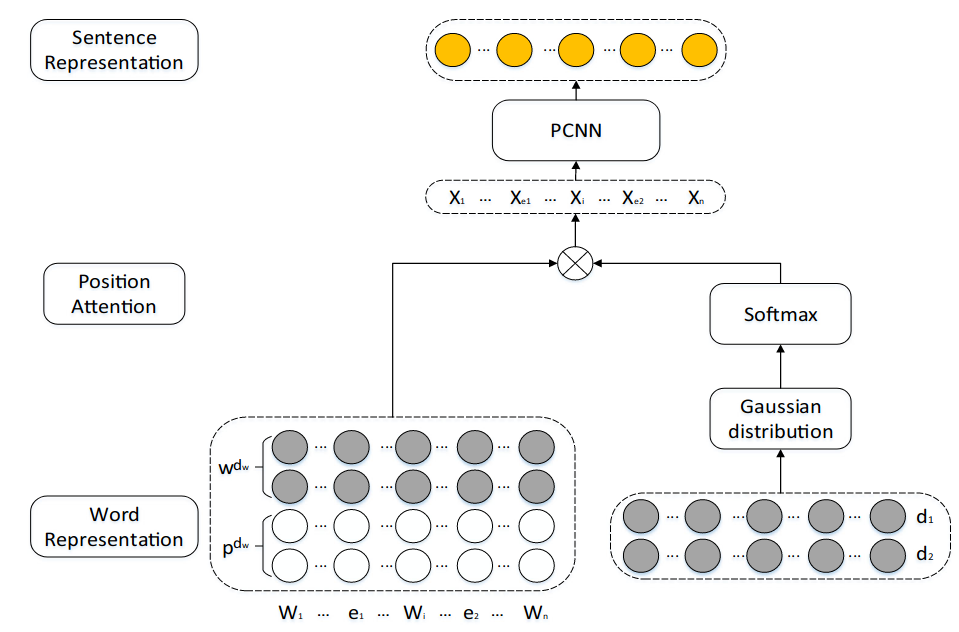
\includegraphics[width=0.8\linewidth]{images/pos_attension/pos_attension.png}
    \caption{مدل بازنمایی جمله}
    \label{pos_attension}
\end{figure}

\subsection{شبکه توجه به دسته‌های با ویژگی‌های مشابه}

مجموعه داده‌ای که برای این پژوهش استفاده شده است، شامل ۵۳ رابطه مختلف است. اما بیشتر برای بیشتر این روابط
تنها یک نمونه وجود دارد. مشخص است که برای چنین دسته‌هایی شبکه قادر نخواهد بود ویژگی‌های مناسبی استخراج کند.
روشی که در این پژوهش ارائه شده است ادغام ویژگی‌های مشابه از دسته‌های دیگر در این شبکه است.

\begin{figure}[h]
    \centering
    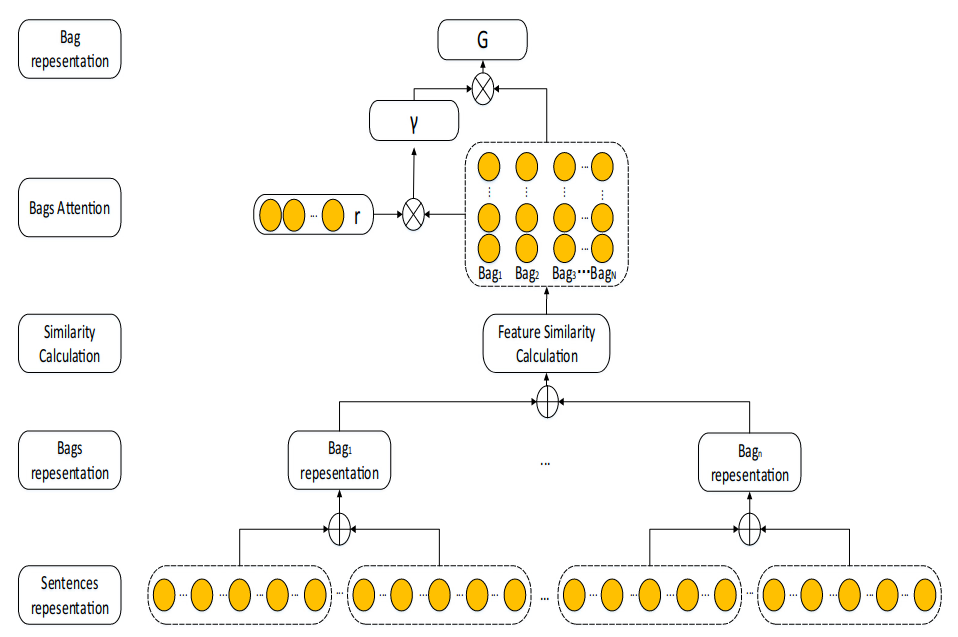
\includegraphics[width=0.8\linewidth]{images/pos_attension/bag_attension.png}
    \caption{ساختار مدل توجه به دسته‌های با ویژگی‌های مشابه}
    \label{bag_attension}
\end{figure}

راهکار ارائه شده به این صورت عمل می‌کند که ابتدا شباهت ویژگی‌های استخراج شده برای دسته فعلی را با ویژگی‌های
تمام دسته‌های دیگر از طریق رابطه‌ی ریاضی زیر محاسبه می‌کنند.

\begin{eqnarray}
    \text{\lr{sim}}(\text{\lr{Bag}}_i, \text{\lr{Bag}}_j) = \text{\lr{Bag}}_i \text{\lr{Bag}}^T_j
\end{eqnarray}

سپس $n$ تا از شبیه‌ترین دسته‌ها انتخاب می‌شود. در قدم بعدی ویژگی‌ها وزن‌دهی شده و بر اساس وزن‌ها
ترکیب می‌شوند. وزن‌های این با استفاده از فرمول زیر استخراج می‌شود.

\begin{eqnarray}
    \gamma_i & = & \frac{\exp(e_i)}{\sum_{k}^{N} \exp(e_k)} \\
    \exp(e_i) & = & \text{\lr{Group}}_i^{j} B r
\end{eqnarray}

در فرمول بالا $B$ یک ماتریس قطری وزن و $r$ یک بازنمایی برداری از رابطه است. پس از محاسبه $\gamma_i$ها ویژگی‌ها
به صورت زیر با هم ترکیب می‌شوند.

\begin{eqnarray}
    G_i = \sum_{i}^{N} \gamma_i \textrm{\lr{Group}}_i^{j}
\end{eqnarray}

برچسب نهایی با استفاده از $G_i$ها تعیین می‌شود.
